\documentclass[floatfix,nofootinbib,superscriptaddress,fleqn,preprint]{revtex4} 
%\documentclass[aps,epsfig,tightlines,fleqn]{revtex4}
\usepackage[utf]{kotex}
\usepackage[HWP]{dhucs-interword}
\usepackage[dvips]{color}
\usepackage{graphicx}
\usepackage{bm}
%\usepackage{fancyhdr}
%\usepackage{dcolumn}
\usepackage{defcolor}
\usepackage{amsmath}
\usepackage{amsfonts}
\usepackage{amssymb}
\usepackage{amscd}
\usepackage{amsthm}
\usepackage[utf8]{inputenc}
 \usepackage{setspace}
%\pagestyle{fancy}

\begin{document}

\title{\Large 2022년 1학기 물리학 I: Quiz 14}
\author{김현철\footnote{Office: 5S-436D (면담시간 매주
    화요일-16:00$\sim$20:00)}} 
\email{hchkim@inha.ac.kr}
\affiliation{Hadron Theory Group, Department of Physics,
Inha University, Incheon 22212, Republic of Korea }
\date{Spring semester, 2022}


\vspace{1.cm}
\begin{abstract}
\noindent \textbf{ {\color{red}주의}: \color{blue} 단 한 번의 부정행위도 절대
  용납하지 않습니다. 적발 시, 학점은 F를 받게 됨은 물론이고,
  징계위원회에 회부합니다. One strike out임을 명심하세요.}\\
\\
문제는 다음 쪽부터 나옵니다.  \\ \\
{\bf Date:} 2022년 4월 27일 (수) 15:30-16:15
\\
{\bf 학번:} \hspace{4cm}
{\bf 이름:} 

\end{abstract}
\maketitle

\noindent {\bf 문제 1. (30 pt)} 
그림~\ref{fig:1}에서 크기가 10 N인 힘이 질량 10 kg이고 반지름이 0.30
m인 바퀴에 수평방향으로 작용하고 있다. 바퀴는 수평면에 대하여 유연한
굴림 운동을 하며 질량중심에 대한 가속도의 크기는 0.60
$\mathrm{m/s^2}$이다. 
\begin{figure}[htp]
  \centering
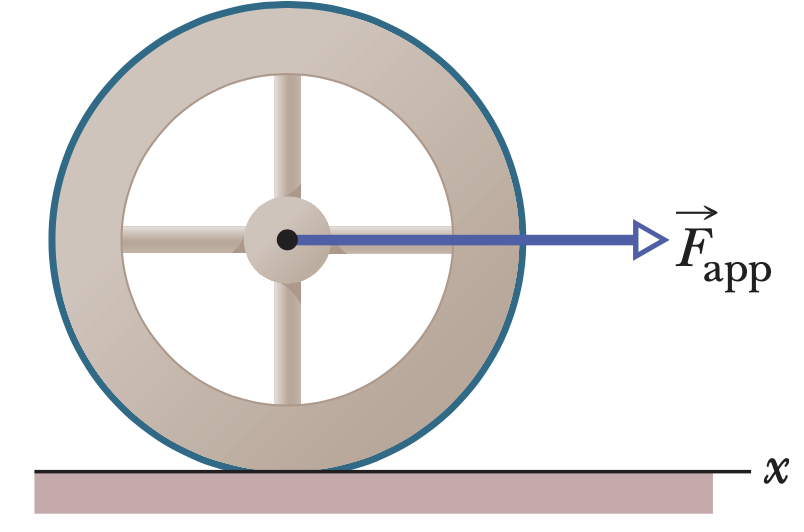
\includegraphics[scale=0.5]{Qfig14-1-20220427.png}
  \caption{문제 1}
  \label{fig:1}
\end{figure}
\begin{itemize}
\item[(가)] 바퀴에 작용하는 마찰력을 단위벡터로 표기하여라.
\item[(나)] 질량중심을 지나는 회전축에 대한 바퀴의 회전관성은
  얼마인가?   
\end{itemize}

 \newpage

{\color{gray} [문제 풀이 쪽]}

\newpage

\noindent {\bf 문제 2. (30 pt)}
그림~\ref{fig:2}는 질량이 $m$, 반지름이 $R$인 원형고리와 질량이 $m$,
길이 $R$인 네 개의 가느다란 막대로 만들어진 정사각형 강체이다. 강체는
주기가 2.5 초인 일정한 속력으로 수직축에 대하여 회전한다. $R=0.50$ cm,
$m=2.0$ kg이라고 할 때,
\begin{figure}[ht]
  \centering
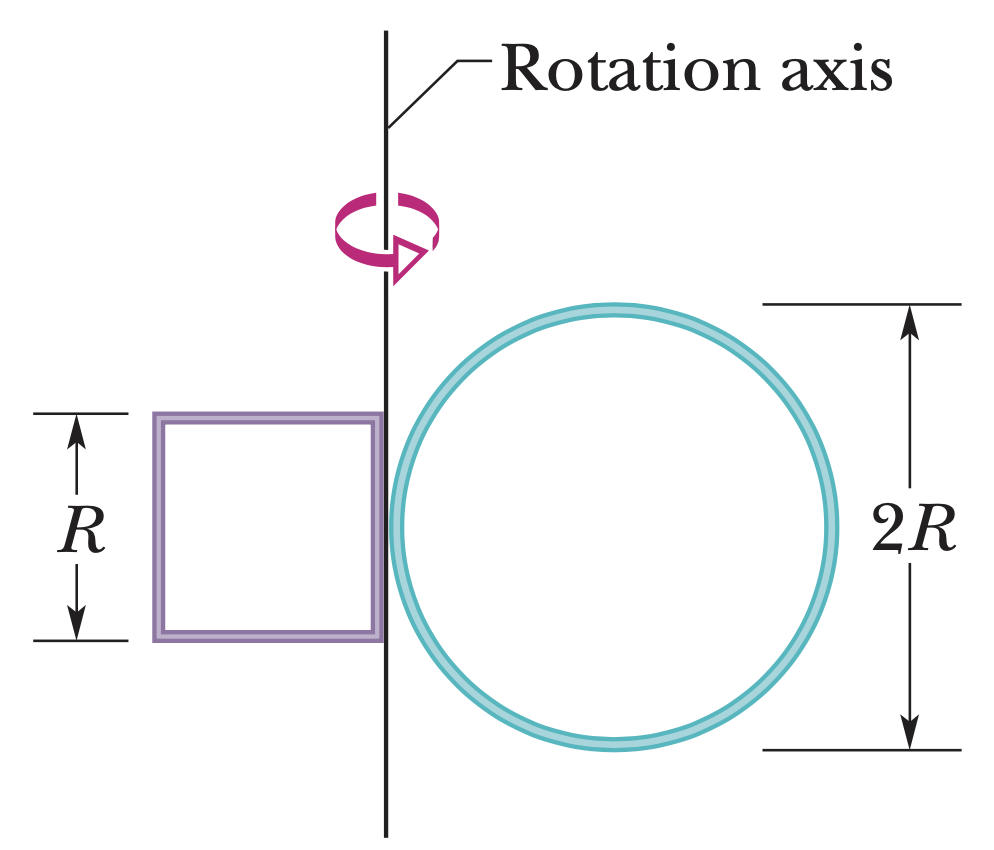
\includegraphics[scale=0.4]{Qfig14-2-20220427.png}
  \caption{문제 2}
  \label{fig:2}
\end{figure}
\begin{itemize}
\item[(가)] 회전축에 대한 강체의 회전관성과
\item[(나)] 회전축에 대한 각운동량을 각각 구하여라.   
\end{itemize}
\newpage
{\color{gray} [문제 풀이 쪽]}

\newpage

\noindent {\bf 문제 3. (40pt)} 
질량이 4.0 kg이고 길이가 0.50 m인 가늘고 균일한 막대가 수평면에서
중심을 지나는 수직축에 대하여 회전할 수 있다. 질량이 3.0 g인 총알이
막대의 회전면에서 정지하고 있는 막대의 왼쪽 끝을 향하여
발사되었다. 위에서 보았을 때 총알의 경로는 그림~\ref{fig:3}처럼 막대와
$\theta=60^\circ$의 각도를 이룬다. 총알이 막대에 박히고 충돌 직후
막대의 가속도가 10 rad/s이라면 충돌 직전 총알의 속력은 얼마인가? 
\begin{figure}[ht]
  \centering
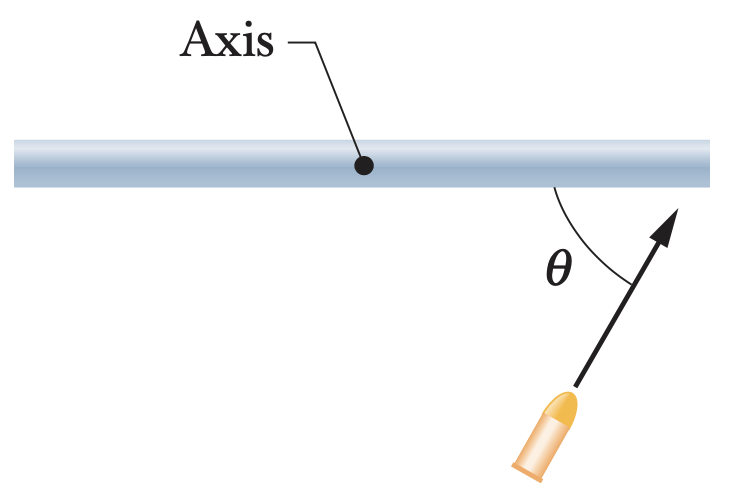
\includegraphics[scale=0.4]{Qfig14-3-20220427.png}
  \caption{문제 3}
  \label{fig:3}
\end{figure}
\newpage
{\color{gray} [문제 풀이 쪽]}

\newpage

\noindent {\bf 문제 4. (60pt) {\color{red} 난이도 상}:}
그림~\ref{fig:4}에서 질량 30 kg의 아이가 질량이 100 kg, 반지름이 2.0
m인 정지해 있는 원판의 가장자리에 서 있다. 원판의 중심에 있는 회전축에
대한 회전관성은 $150\,\mathrm{kg\cdot m^2}$이다. 이때 친구가 던진
질량이 1.0 kg인 공을 아이가 잡았다. 공을 잡기 직전에 수평방향인 공의
속도 $\vec{v}$의 크기는 12 m/s이고 원판의 가장자리의 접선과
$\vec{v}$가 이루는 각도는 $37^\circ$이다. 아이가 공을 잡은 직후 원판의
각속력을 구하여라. 
\begin{figure}[ht]
  \centering
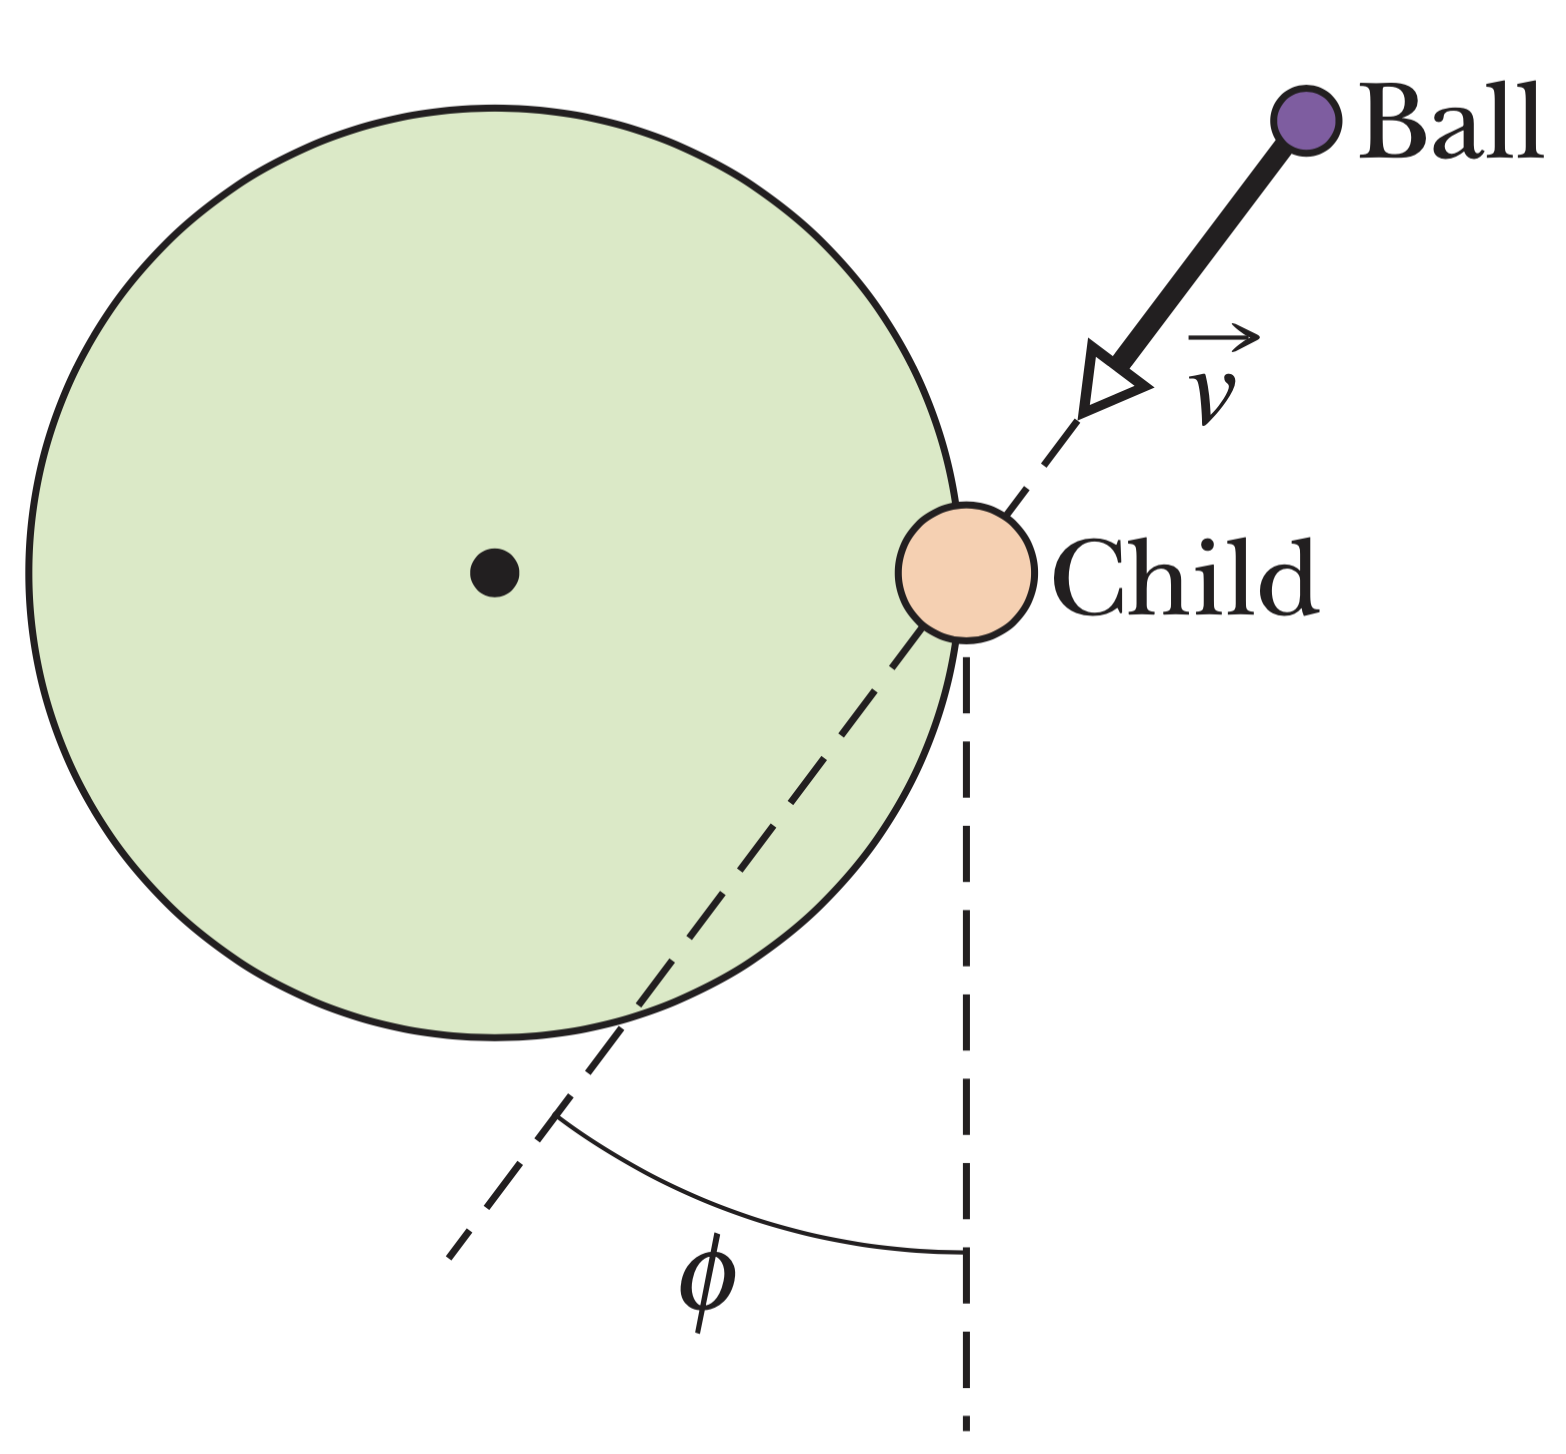
\includegraphics[scale=0.25]{Qfig14-4-20220427.png} 
  \caption{문제 4}
  \label{fig:4}
\end{figure}
\newpage
{\color{gray} [문제 풀이 쪽]}

\newpage
\end{document}